\documentclass[]{IEEEtran}

% Your packages go here
\usepackage[utf8]{inputenc}
\usepackage{graphicx}
\usepackage{float}
\usepackage{listings}
\usepackage{xcolor}
\usepackage{mathrsfs}
\usepackage{amsmath}
%listings settings
\definecolor{codegreen}{rgb}{0,0.6,0}
\definecolor{codegray}{rgb}{0.5,0.5,0.5}
\definecolor{codepurple}{rgb}{0.58,0,0.82}
\definecolor{backcolour}{rgb}{0.95,0.95,0.92}
\definecolor{codeblue}{rgb}{0,0.8,0.99}
\definecolor{codeyellow}{rgb}{0.6,0.5,0}


\lstdefinestyle{vim_like}{
  backgroundcolor=\color{backcolour},   
  commentstyle=\color{codegreen},
  keywordstyle=\color{codeyellow},
  numberstyle=\tiny\color{codegray},
  stringstyle=\color{codepurple},
  basicstyle=\ttfamily\footnotesize,
  breakatwhitespace=false,         
  breaklines=true,                 
  captionpos=b,                    
  keepspaces=true,                 
  numbers=left,                    
  numbersep=5pt,                  
  showspaces=false,                
  showstringspaces=false,
  showtabs=false,                  
  tabsize=2
}
\lstset{style=vim_like}

\markboth{MO443 Digital Image Processing}{}

\begin{document}
  \title{Project 2 - Thresholding}
  \author{Thales Mateus Rodrigues Oliveira (RA 148051)
    \thanks{ra148051@students.ic.unicamp.br}
  }
  \maketitle
  
  \begin{abstract}
    In this project, it was given the task of applying global and local threshold methods to grayscale images. To fulfill the requirements, the solution implements 8 different algorithms, using approaches listed in the literature. It was able to generate the binarized thresholded images, and the differences of each approach, the pros and cons of the implementation are explained in this report.
  \end{abstract}
  
\section{Introduction}
Thresholding is a technique used for segmentation, and consists on the classification of the pixels within an image according to a(some) specific threshold(s). It is used for basic segmentation, to be able to separate objects from brackground in images and make it easier image processing steps. There are global techiniques, which considers one (or more) general threshold(s) for the entire picture, and local ones, that calculates local threshold(s) for every region in the image. The goal of this work is to implement global and local approaches, and be able to compare their strenghts and weakness. The next sections explains the implemented algorithm, the experiments realized and the output analysis
\par The code, along with the input files and the report is delivered in the compressed file THALES\_MATEUS\_RODRIGUES\_OLIVEIRA\_148051.tar, in the Google Classroom.
\section{The Program}
 
The program was implemented with Python 3.7.3. The libraries used and their respective versions are OpenCV 4.1.0, Numpy 1.16.4 and MatPlotLib 3.1.0.

\subsection{How to execute it}

The project has a Makefile available to help performing some actions on it. The Makefile has 3 basic instructions: clean, build and exec. Clean instruction removes generated images stored in the \textbf{output} folder, the execution code in \textbf{bin} folder and the folders itself. The Build instruction creates the \textbf{output} and \textbf{bin} folders, and moves the source code to \textbf{bin}. The Exec instruction executes the code with images in the \textbf{input} folder. Listing \ref{code:makefile} provides examples of how to execute the three instructions in a terminal.
\begin{lstlisting}[language=sh, caption={Makefile usage example}, label={code:makefile}]
  #clean environment, deletes output and bin folders and their content
  make clean
  
  #prepare the environment for code execution
  make build 

  #executes code
  make exec
\end{lstlisting}

\subsection{Input}

The program does not have an input argument by default, the input images are listed in code, and they are expected to be stored in the \textbf{input} folder. Listing \ref{code:input} shows how images are listed to be executed in code. The $images$ tuple is implemented in $src/main.py$.
\par The images are expected to be in the \textit{.pgm} format.

\begin{lstlisting}[language=Python, caption={Input images inside code}, label={code:input}]
  # for inserting other images, add tem to /input folder and list them here
  images = (
      'baboon',
      'fiducial',
      'monarch',
      'peppers',
      'retina',
      'sonnet',
      'wedge'
  )
\end{lstlisting}

\subsection{Output}
The output of the program is a series of binarized images based on the input ones, threshold methods and their peculiarities, and their respective histograms. The output images are stored in the \textbf{output} folder, and they stored based on global or local threshold methods (\textbf{global-thresholding} and \textbf{nxn-window} folders) and are labeled by concatenating the image name and the threshold method, for local cases (\textit{e.g.: output/99x99-window/baboon\_bernsen.pgm}). The histograms of the images are stored following the same convention (\textit{e.g.: output/99x99-window/fiducial\_contrast\_histogram.pgm}). The ratio of black (object) pixels in each image is also an output of the program, using the standard output. 

\subsection{Implementation}
The functions which implement the thresholding operations are defined in the \textit{src/thresholding.py} file. The file has an auxiliary function to build histograms for images \textit(calculate\_histogram), and has 8 thresholding functions, 1 for the global method and 7 other to the local approaches. The thresholding methods were implemented according to the project specification. For some local methods, as they deal with neighborhood centered in the analyzed pixel, the image is padded according to the neighborhood size. The convention here applied is that background pixels have maximum value (255) and object pixels have minimum value (0). The following items describe each of the used approaches.

\subsubsection{Global Thresholding}
The value of each image pixel is compared to a threshold. If greater than the threshold, it is an object pixel. Otherwise, it is background. It is the simpler method, and the used threshold is received as an input for the function. Listing \ref{code:global} shows the most important lines of the implementation.

\begin{lstlisting}[language=Python, caption={Global Thresholding Implementation}, label={code:global}]
def global_thresholding(img, threshold=128):
  ...
  result = np.where(img < threshold, 255, 0)
  result = np.uint8(result)
  ...
\end{lstlisting}

\subsubsection{Bernsen Thresholding}
The Bernsen approach for local thresholding calculates the threshold of a specific pixel based on the mean of the maximum and minimum values of its neighborhood centered in the pixel. Then, the comparison to set the value is done. Listing \ref{code:bernsen} shows the most important lines of the implementation.

\begin{lstlisting}[language=Python, caption={Bernsen Local Thresholding Implementation}, label={code:bernsen}]
  def bernsen_local_thresholding(img, window_size=3):
    ...
    padded_img = np.pad(img, (window_size//2, window_size//2), 'constant')
    for j in range(img_height):
        for i in range(img_width):
            window = padded_img[j:j + window_size, i:i + window_size]
            local_threshold = (int(np.min(window)) + int(np.max(window)))//2
            if img[j][i] < local_threshold:
                result[j][i] = 255
    ...
\end{lstlisting}

\subsubsection{Niblack Thresholding}
The Niblack approach for local thresholding is based on the pixel's neighborhood mean and standard deviation values. The threshold is calculated as:
\begin{equation}
  T(x, y) = \mu(x, y) + k\sigma(x,y) 
\end{equation}
where $\mu$,$\sigma$ are the mean and standard deviation in the neighborhood, respectively, and $k$ an adjustment factor. The literature calculates a good value of $k$ as $0.2$. Listing \ref{code:niblack} shows the main lines of the implementation.

\begin{lstlisting}[language=Python, caption={Niblack Local Thresholding Implementation}, label={code:niblack}]
  def niblack_local_thresholding(img, window_size=15, k=-0.2):
    ...
    for j in range(img_height):
        for i in range(img_width):
        window = img[window_size*(j//window_size):window_size*(j//window_size) + window_size,
        window_size*(i//window_size):window_size*(i//window_size) + window_size]
          mean = np.mean(window)
          std_dev = np.std(window)
          local_threshold = int(mean + k*std_dev)
          if img[j][i] < local_threshold:
              result[j][i] = 255
    ...
\end{lstlisting}

\subsubsection{Sauvola and Pietaksinen Thresholding}
This solution tries to improve Niblack one, specially for documents with bad lighting. The threshold is calculated as:

\begin{equation}
  T(x,y) = \mu (x,y)*(1 + k(\dfrac{\sigma(x,y)}{R} - 1))
\end{equation}

The standard deviation and mean are calculated based on neighborhood centered in the analyzed pixel. Listing \ref{code:sauvola} shows main parts of implementation. The default $k$ and $R$ values are suggestions from the creators.

\begin{lstlisting}[language=Python, caption={Sauvola and Pietaksinen Local Thresholding Implementation}, label={code:sauvola}]
  def sauvola_pietaksinen_local_thresholding(img, window_size=3, k=0.5, r=128):
    ...
    padded_img = np.pad(img, (window_size//2, window_size//2), 'constant')
    img_height, img_width = img.shape
    for j in range(img_height):
        for i in range(img_width):
            window = padded_img[j:j + window_size, i:i + window_size]
            mean = np.mean(window)
            std_dev = np.std(window)
            local_threshold = int(mean*(1 + k*((std_dev/r) - 1)))
            if img[j][i] < local_threshold:
                result[j][i] = 255
    ...
\end{lstlisting}

\subsubsection{Phansalskar, More and Sabale Thresholding}
This approach is a variation of Sauvola and Pietaksinen, to deal with low cotnrast images. The calculation of threshold for local neighborhood is done as:
\begin{equation}
  T(x, y) = \mu(x,y)*(1 + pexp(-q\mu(x,y)) + k*(\dfrac{\sigma(x,y)}{R} - 1))
\end{equation}

The $p, q, k, R$ default parameters are suggested from the authors as $2, 10, 0.25 and 0.5$, respectively. The calculation is done for normalized image. Listing \ref{code:more} shows the main aspects of the implementation. 

\begin{lstlisting}[language=Python, caption={Phansalskar, More and Sabale Local Thresholding Implementation}, label={code:more}]
  def phansalskar_more_sabale_local_thresholding(img, window_size=3, k=0.25, r=0.5, p=2, q=10):
    ...
    for j in range(img_height):
        for i in range(img_width):
            window = img[window_size*(j//window_size):window_size*(j//window_size) + window_size,
                         window_size*(i//window_size):window_size*(i//window_size) + window_size]
            # image is normalized
            window = window/255
            mean = np.mean(window)
            std_dev = np.std(window)
            local_threshold = (mean*(1 + (p*math.exp(-q*mean)) + (k*(((std_dev)/r) - 1))))
            if img[j][i]/255 < local_threshold:
                result[j][i] = 255
    ...
\end{lstlisting}

\subsubsection{Contrast Thresholding}
This solution analyzes de distance of the pixel value to the min and max values of the local neighborhood. If it is closer to the max, it is part of the object. It is background, otherwise. Listing \ref{code:contrast} clarifies the implementation.

\begin{lstlisting}[language=Python, caption={Contrast Thresholding Implementation}, label={code:contrast}]
  def contrast_local_thresholding(img, window_size=3):
    ...
    for j in range(img_height):
        for i in range(img_width):
            window = img[window_size*(j//window_size):window_size*(j//window_size) + window_size,
                         window_size*(i//window_size):window_size*(i//window_size) + window_size]
            min_v = np.min(window)
            max_v = np.max(window)
            dist_min = abs(min_v - int(img[j][i]))
            dist_max = abs(max_v - int(img[j][i]))
            if dist_min < dist_max:
                result[j][i] = 255
    ...
\end{lstlisting}

\subsubsection{Mean Thresholding}
This approach sets the threshold as the mean of the local neighborhood of the analyzed pixel. Listing \ref{code:mean} shows the main aspects of the implementation.

\begin{lstlisting}[language=Python, caption={Mean Thresholding Implementation}, label={code:mean}]
  def mean_local_thresholding(img, window_size=3):
    ...
    for j in range(img_height):
        for i in range(img_width):
            window = img[window_size*(j//window_size):window_size*(j//window_size) + window_size,
                         window_size*(i//window_size):window_size*(i//window_size) + window_size]
            mean = np.mean(window)
            if img[j][i] < mean:
                result[j][i] = 255
    ...
\end{lstlisting}

\subsubsection{Median Thresholding}
The solution sets the threshold as the median of the local neighborhood of the analyzed pixel. Listing \ref{code:median} shows main parts of implementation.

\begin{lstlisting}[language=Python, caption={Median Thresholding Implementation}, label={code:median}]
  def median_local_thresholding(img, window_size=3):
    ...
    for j in range(img_height):
        for i in range(img_width):
            window = img[window_size*(j//window_size):window_size*(j//window_size) + window_size,
                         window_size*(i//window_size):window_size*(i//window_size) + window_size]
            median = np.median(window)
            if img[j][i] < median:
                result[j][i] = 255
    ...
\end{lstlisting}

\section{Experiments}
The \textit{src/main.py} file executes the test pipeline. The idea is the following: for each input image, for each global threshold, execute the global thresholding method. For each window size, executes all local thresholding methods listed prior. For each global and local executions, save the output images and their respective histograms. Also, print in the standard output the ratio of black (object) pixels. The input images are stored in \textbf{input} folder as mentioned before, and their names and dimensions are listed in table \ref{table:input}. The input images are shown in figure \ref{fig:input-images}. The generated output images for the report are saved in $png$ extension in order to make it easier the report manipulation, and are stored in the report folder.

\begin{table}[h!]
\centering
\begin{center}
\begin{tabular}{ |c|c| } 
 \hline
 Image Names & Dimensions (width x height) \\
 \hline
  baboon.pgm &  512 x 512\\ 
 \hline
  fiducial.pgm & 640 x 480\\
 \hline
  monarch.pgm &  768 x 512\\ 
 \hline
  peppers.pgm & 623 x 594\\
 \hline
 retina.pgm & 256 x 256\\
 \hline
 sonnet.pgm & 384 x 510\\
 \hline
 wedge.pgm & 507 x 384\\
 \hline
\end{tabular}
\caption{Input images used in experiments}
\label{table:input}
\end{center}
\end{table}

\begin{figure}[H]
  \centering
  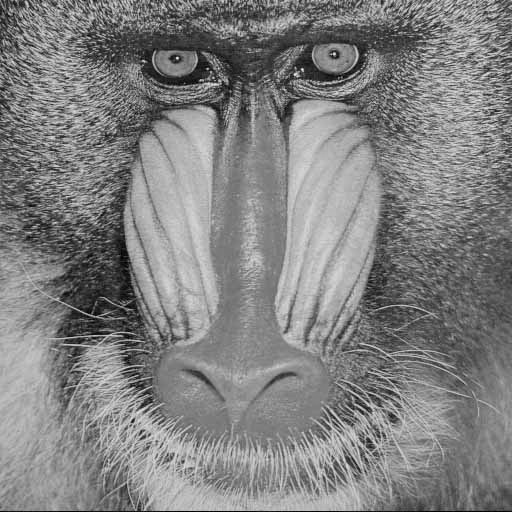
\includegraphics[width=0.2\hsize]{images/baboon.png}
  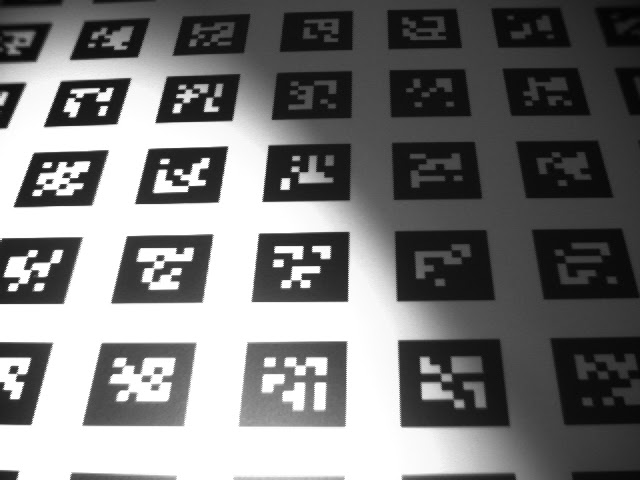
\includegraphics[width=0.2\hsize]{images/fiducial.png}
  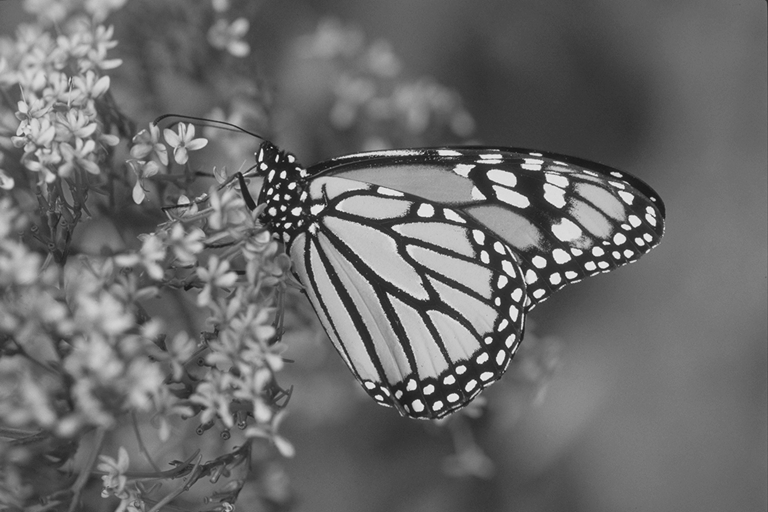
\includegraphics[width=0.2\hsize]{images/monarch.png}
  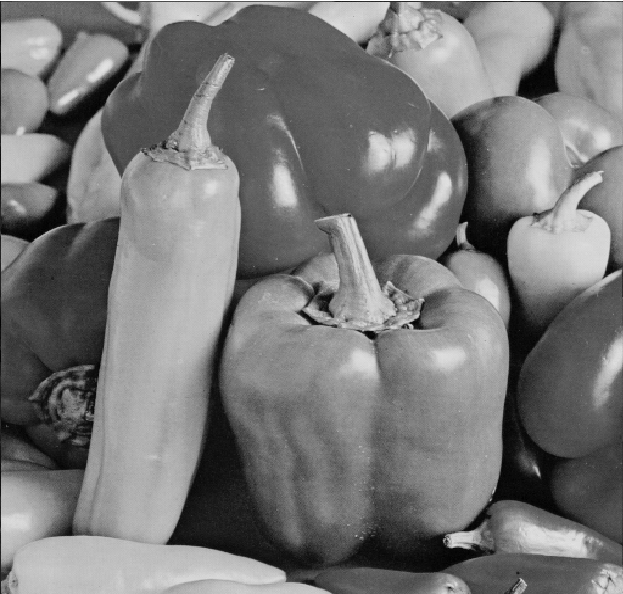
\includegraphics[width=0.2\hsize]{images/peppers.png}
  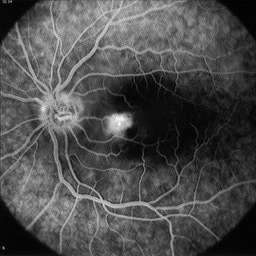
\includegraphics[width=0.2\hsize]{images/retina.png}
  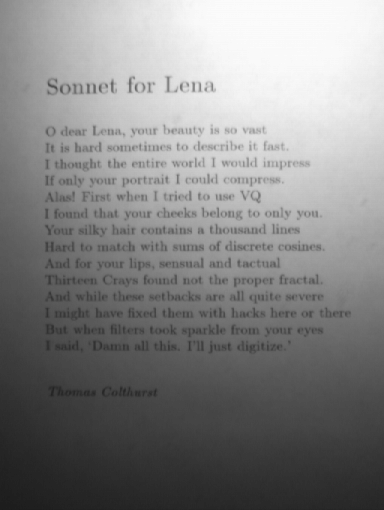
\includegraphics[width=0.2\hsize]{images/sonnet.png}
  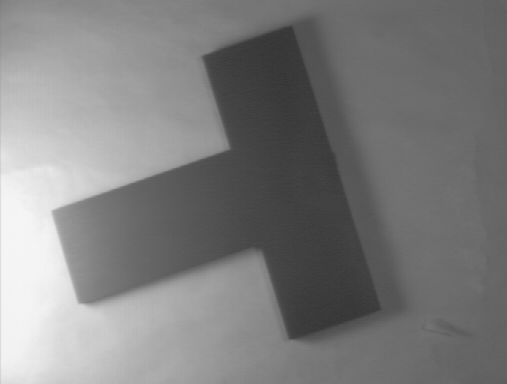
\includegraphics[width=0.2\hsize]{images/wedge.png}
  \caption{Input images used in experiments. a) Baboon. b) Fiducial c) Monarch d) Peppers e) Retina f) Sonnet g) Wedge}
  \label{fig:input-images}
\end{figure}

The images original histogram are also shown in Figure \ref{fig:original-histograms}. They provide a good description of the input images. The Baboon image, which focus on the face of the animal, has a good number of details. The Fiducial image has a "almost binarized" appearance, with values concentrated in the extremes (either black or white, with high concentration of white), and also has some shading (as seen in intermediate values of the histogram). The monarch image has a concentration of intensities in the first half of the spectrum ($[0, 128]$), and it might be difficult to distinguish the butterfly from the background. The peppers image has good, and it might be difficult to separate objects from background. The retina image also has a high concentration of intensities in the first half of the spectrum. The sonnet one has variety of intensities, and some bad lighting in the text. The wedge image has high occurence of middle intensities.

\begin{figure}[H]
  \centering
  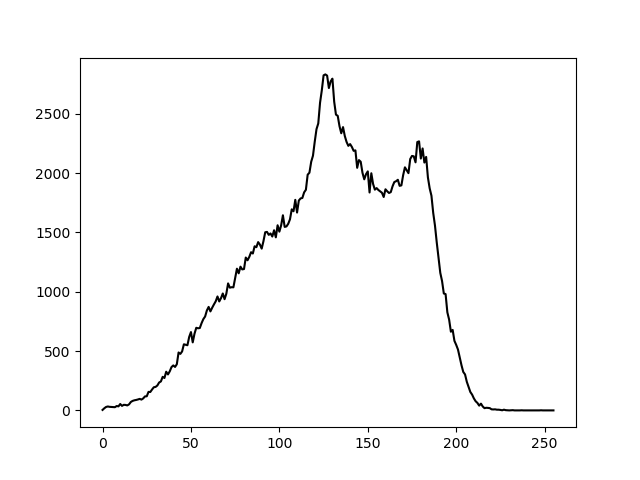
\includegraphics[width=0.3\hsize]{images/-original-histogram-baboon.png}
  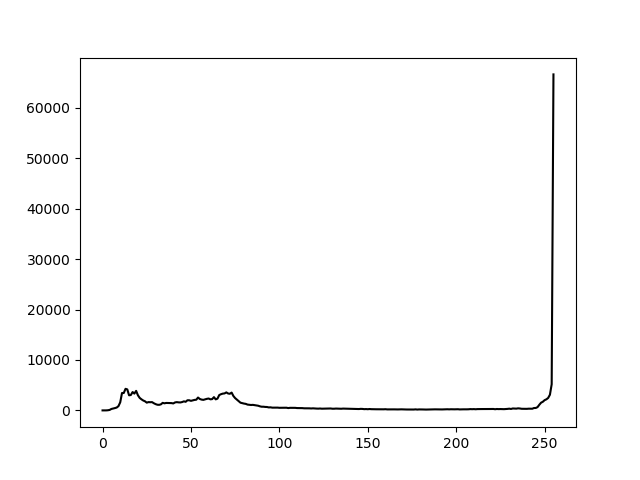
\includegraphics[width=0.3\hsize]{images/-original-histogram-fiducial.png}
  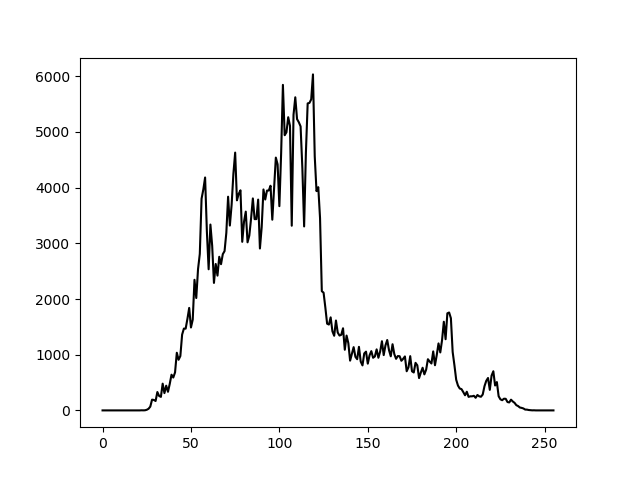
\includegraphics[width=0.3\hsize]{images/-original-histogram-monarch.png}
  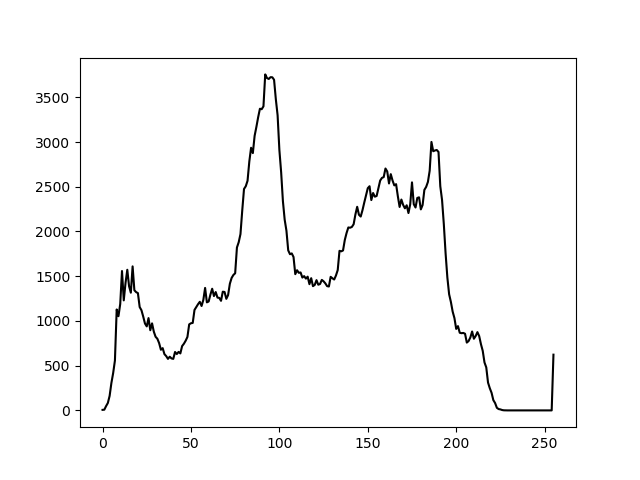
\includegraphics[width=0.3\hsize]{images/-original-histogram-peppers.png}
  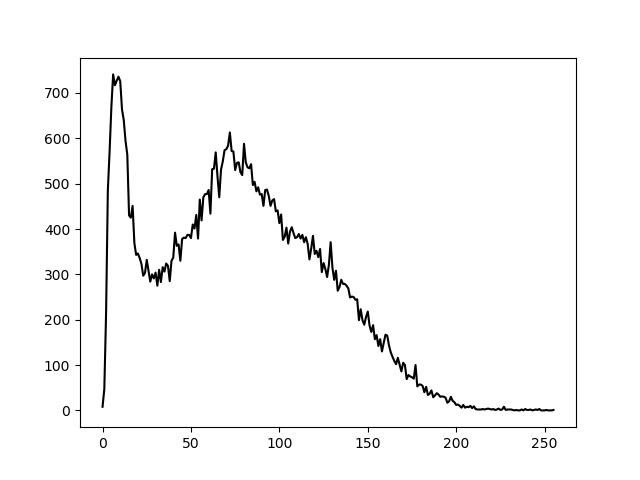
\includegraphics[width=0.3\hsize]{images/-original-histogram-retina.png}
  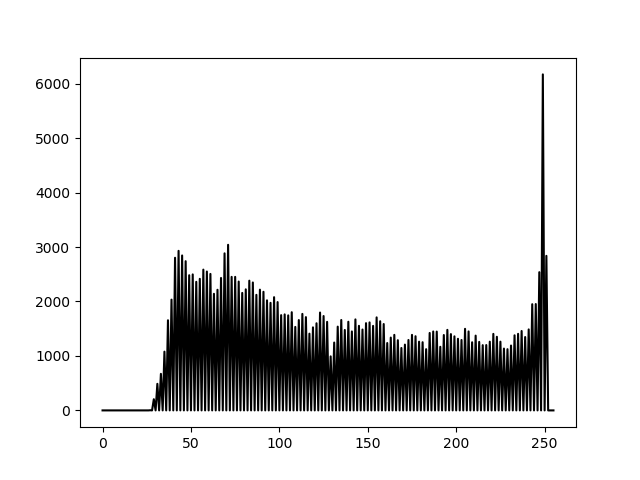
\includegraphics[width=0.3\hsize]{images/-original-histogram-sonnet.png}
  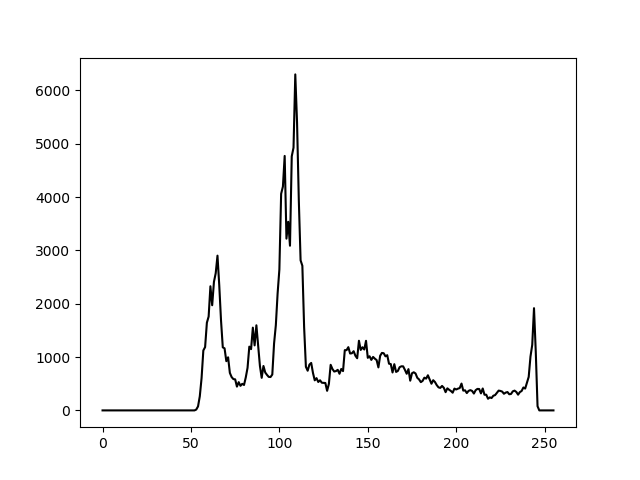
\includegraphics[width=0.3\hsize]{images/-original-histogram-wedge.png}
  \caption{Histogram of input images used in experiments. a) Baboon. b) Fiducial c) Monarch d) Peppers e) Retina f) Sonnet g) Wedge}
  \label{fig:original-histograms}
\end{figure}

For the global thresholding method, values in the $[0,255]$ scale were chosen. Table \ref{table:globalth} lists the global threshold valus used.

\begin{table}[h!]
  \centering
  \begin{center}
  \begin{tabular}{ |c| } 
   \hline
   Global Threshold values \\
   \hline
      50\\ 
   \hline
      128\\
   \hline
      200\\
    \hline
  \end{tabular}
  \caption{Global threshold values used in experiments}
  \label{table:globalth}
  \end{center}
  \end{table}

For the window sizes, a variety of values were picked. The neighborhood is chosen to be always a squared $nxn$ region, where n is the given size.
Table \ref{table:windows} lists the picked values.

\begin{table}[h!]
  \centering
  \begin{center}
  \begin{tabular}{ |c| } 
   \hline
   Window sizes (pixels)\\
   \hline
      3x3\\ 
   \hline
      9x9\\
   \hline
      15x15\\
    \hline
    33x33\\
    \hline
    99x99\\
    \hline
  \end{tabular}
  \caption{Window sizes for selecting pixel's neighborhood}
  \label{table:windows}
  \end{center}
  \end{table}

As we have 7 input images, 3 global threshold methods, 7 local threshold methods and 5 window sizes, we have 266 images of output, and their respective histograms. The output images are stored and well organized in the \textbf{output} folder.

\section{Discussion}
This section is organized in three parts. The first part analyses global thresholding methods and their effectiveness. The second part takes into consideration each local thresholding method, varying the window size. The third one does the comparisons between the local thresholding methods.

\subsection{Global threshold techniques}
In order to analyze the output images for the global threshold techniques, the following images are shown, comparing the thresholded images with different threshold values. The figures \ref{fig:global-fiducial}, \ref{fig:global-monarch}, \ref{fig:global-sonnet} shows the output images for the threshold values ($50$, $128$, $200$).

\begin{figure}[H]
  \centering
  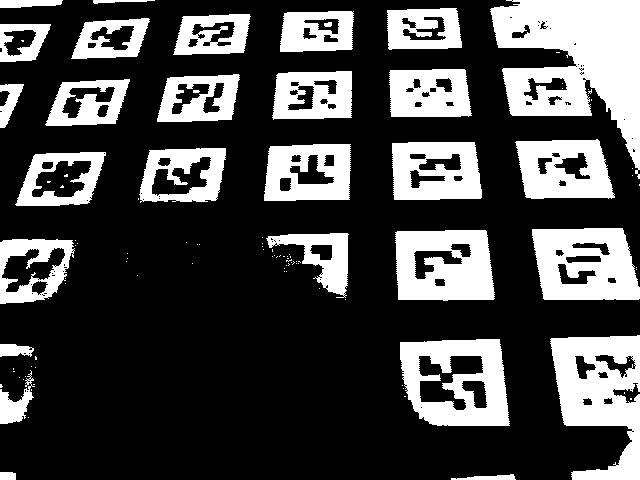
\includegraphics[width=0.3\hsize]{images/global-thresholding/50-threshold/fiducial.png}
  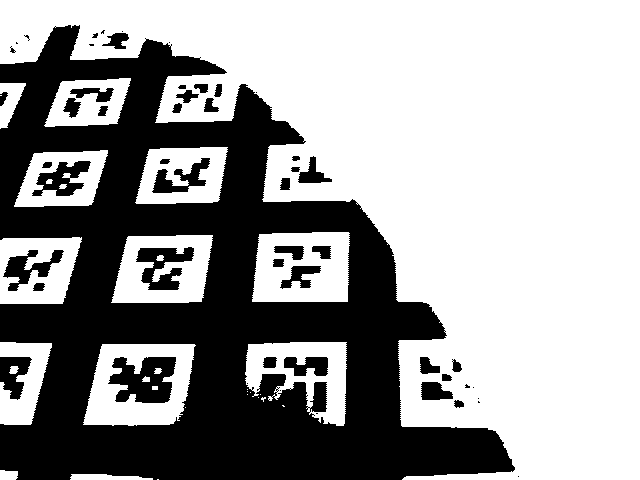
\includegraphics[width=0.3\hsize]{images/global-thresholding/128-threshold/fiducial.png}
  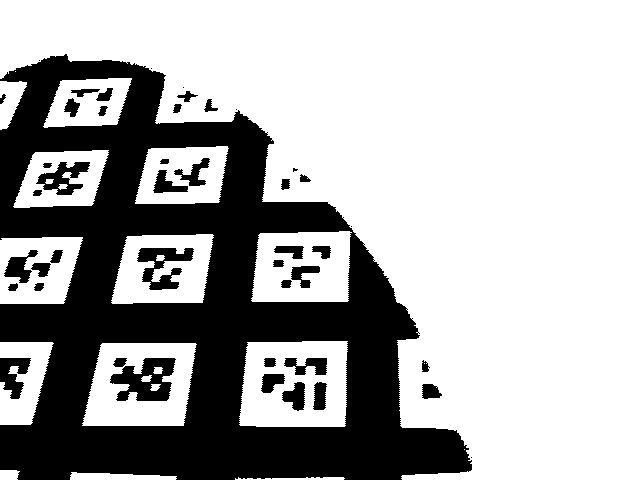
\includegraphics[width=0.3\hsize]{images/global-thresholding/200-threshold/fiducial.png}
  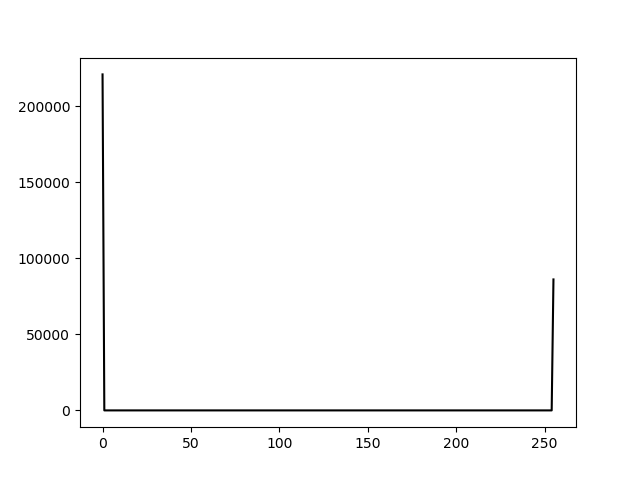
\includegraphics[width=0.3\hsize]{images/global-thresholding/50-threshold/fiducialhistogram.png}
  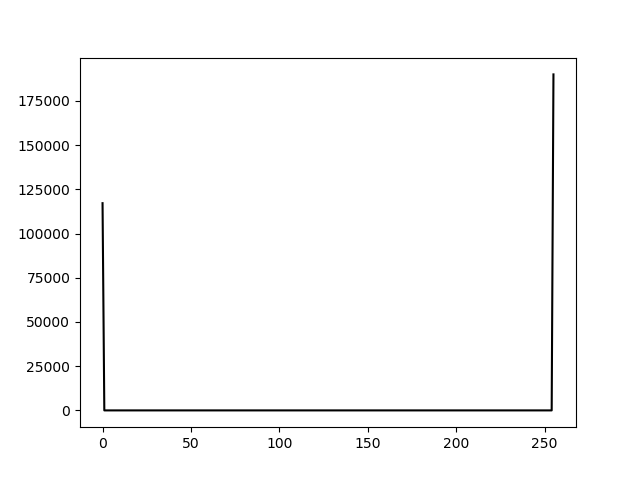
\includegraphics[width=0.3\hsize]{images/global-thresholding/128-threshold/fiducialhistogram.png}
  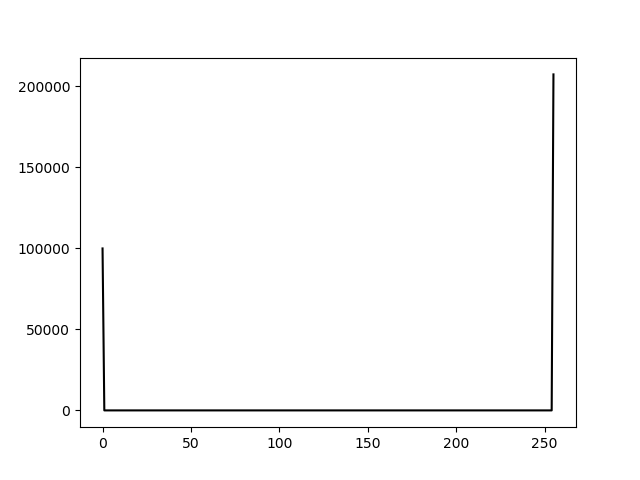
\includegraphics[width=0.3\hsize]{images/global-thresholding/200-threshold/fiducialhistogram.png}
  \caption{Fiducial images with global threshold applying a) Global threshold equals 50. b) Global threshold equals 128. c) Global threshold equals 200. d)Histogram for value 50 e)Histogram for value 128 f)Histogram for value 200}
  \label{fig:global-fiducial}
\end{figure}


\begin{figure}[H]
  \centering
  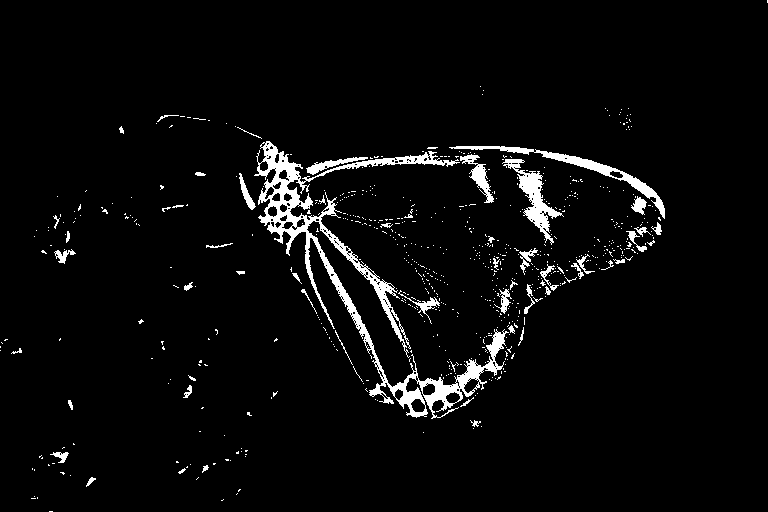
\includegraphics[width=0.3\hsize]{images/global-thresholding/50-threshold/monarch.png}
  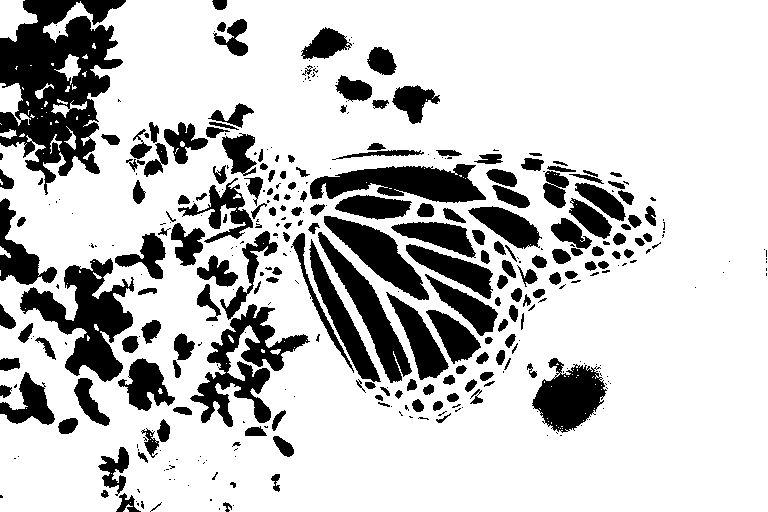
\includegraphics[width=0.3\hsize]{images/global-thresholding/128-threshold/monarch.png}
  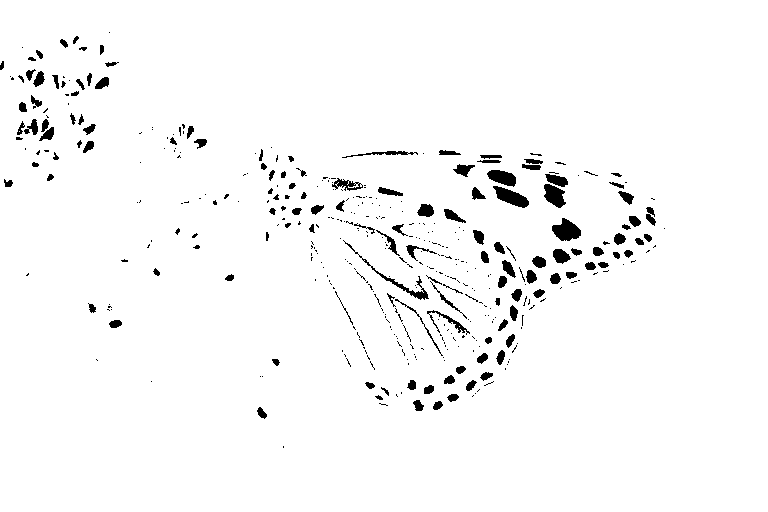
\includegraphics[width=0.3\hsize]{images/global-thresholding/200-threshold/monarch.png}
  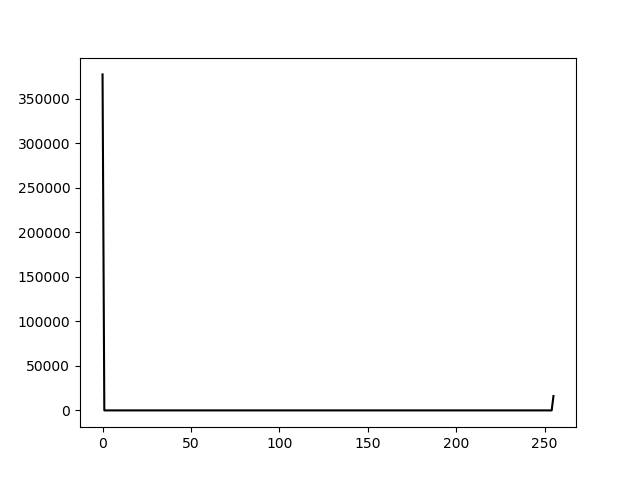
\includegraphics[width=0.3\hsize]{images/global-thresholding/50-threshold/monarchhistogram.png}
  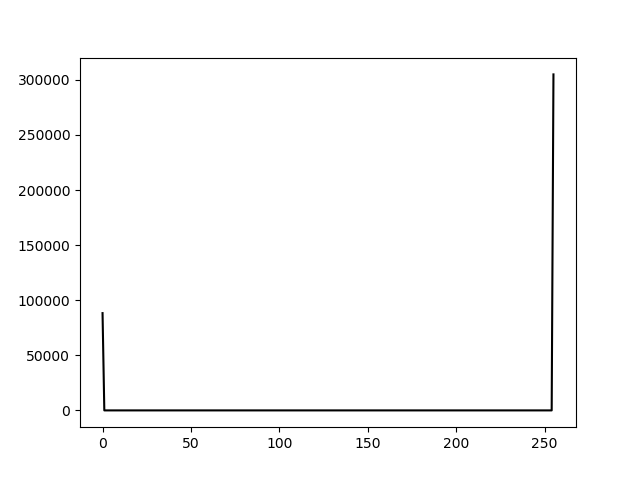
\includegraphics[width=0.3\hsize]{images/global-thresholding/128-threshold/monarchhistogram.png}
  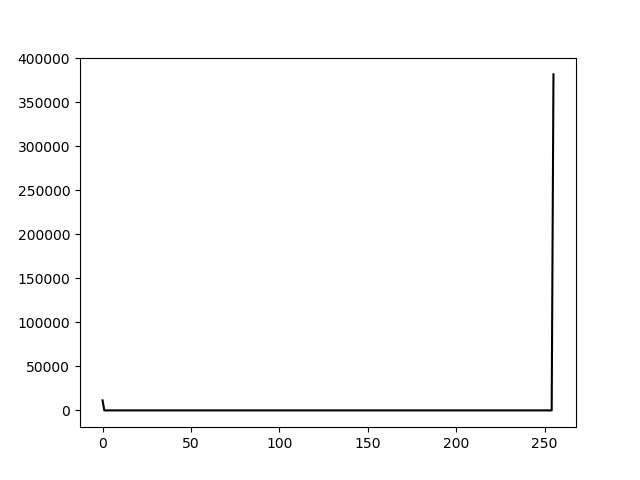
\includegraphics[width=0.3\hsize]{images/global-thresholding/200-threshold/monarchhistogram.png}
  \caption{Monarch images with global threshold applying a) Global threshold equals 50. b) Global threshold equals 128. c) Global threshold equals 200. d)Histogram for value 50 e)Histogram for value 128 f)Histogram for value 200}
  \label{fig:global-monarch}
\end{figure}

\begin{figure}[h]
  \centering
  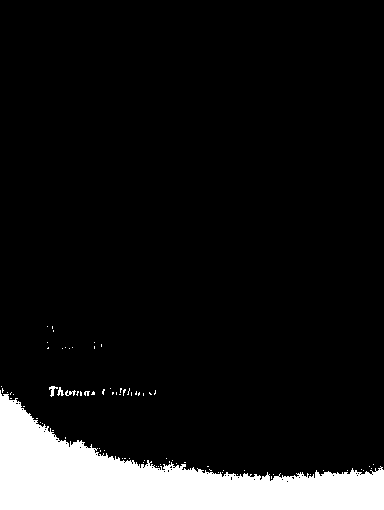
\includegraphics[width=0.3\hsize]{images/global-thresholding/50-threshold/sonnet.png}
  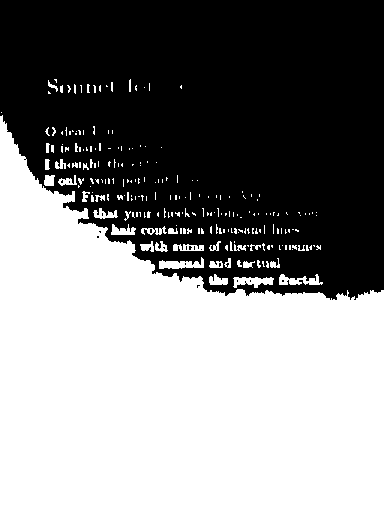
\includegraphics[width=0.3\hsize]{images/global-thresholding/128-threshold/sonnet.png}
  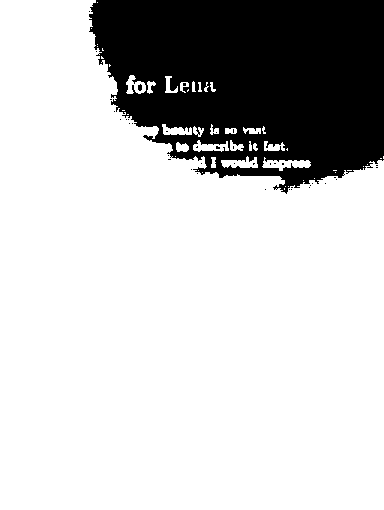
\includegraphics[width=0.3\hsize]{images/global-thresholding/200-threshold/sonnet.png}
  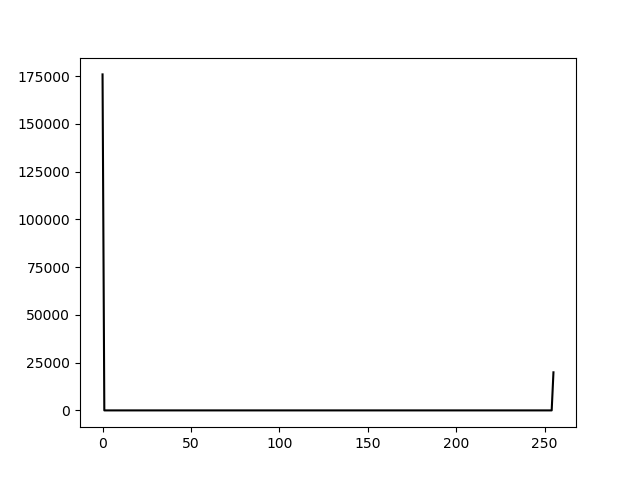
\includegraphics[width=0.3\hsize]{images/global-thresholding/50-threshold/sonnethistogram.png}
  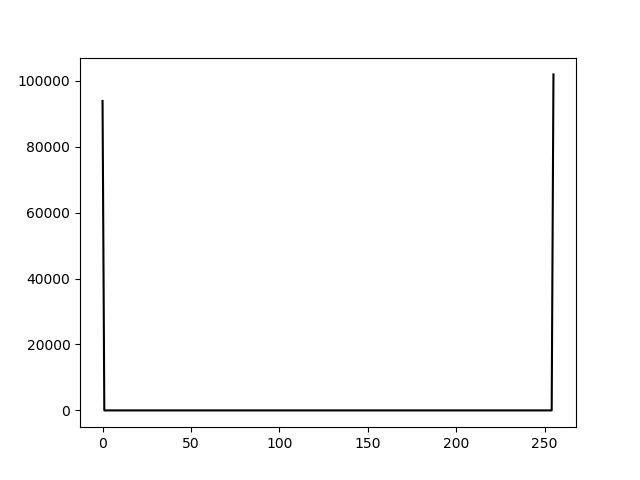
\includegraphics[width=0.3\hsize]{images/global-thresholding/128-threshold/sonnethistogram.png}
  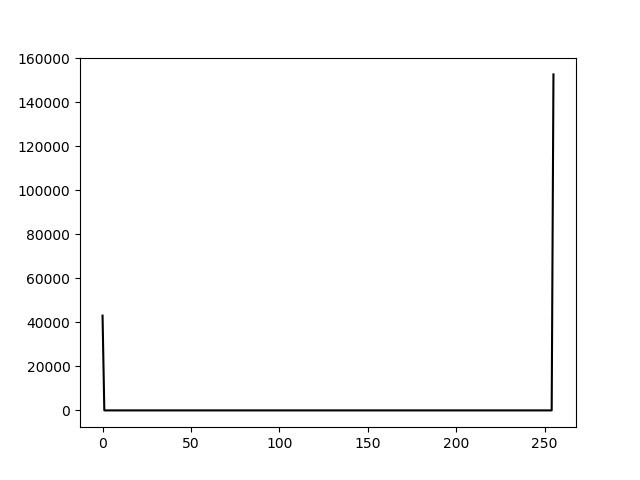
\includegraphics[width=0.3\hsize]{images/global-thresholding/200-threshold/sonnethistogram.png}
  \caption{Sonnet images with global threshold applying a) Global threshold equals 50. b) Global threshold equals 128. c) Global threshold equals 200. d)Histogram for value 50 e)Histogram for value 128 f)Histogram for value 200}
  \label{fig:global-sonnet}
\end{figure}

As expected, even though the global method is able to distinguish background from objects, it does not perform well for any of the thresholds and input images (except for 128 threshold with monarch images). It is does not take into consideration local variations of details and lightning, it cannot identify situations such as shading (for fiducial and sonnet) and any of the threshold values is good enough to separate the text from the background for the sonnet one. As it can be seen from the respective histograms, the number of pixels classified as objects increases as the threshold value is increased. This might not be adequate for images in general.

\subsection{Local Thresholding}

\subsubsection{Bernsen Method}
 For the Bernsen method, the Figure \ref{fig:local-bernsen-baboon} illustrates the obtained results for the baboon image. As shown from the histograms, the ratios of object pixels stays similar from one neighborhood size to the other, selecting more uniform areas as the window size gets bigger. 
\begin{figure}[h]
  \centering
  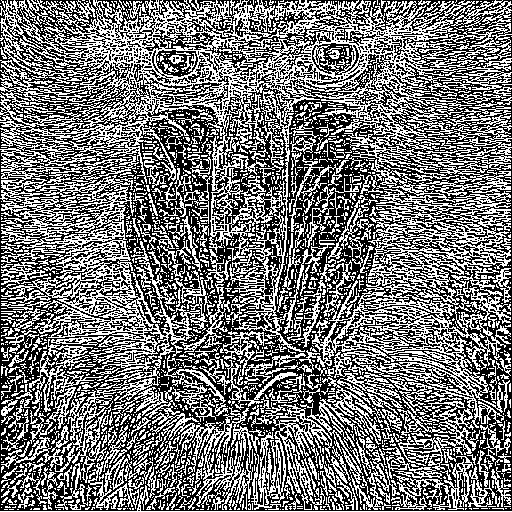
\includegraphics[width=0.3\hsize]{images/3x3-window/baboon_bernsen.png}
  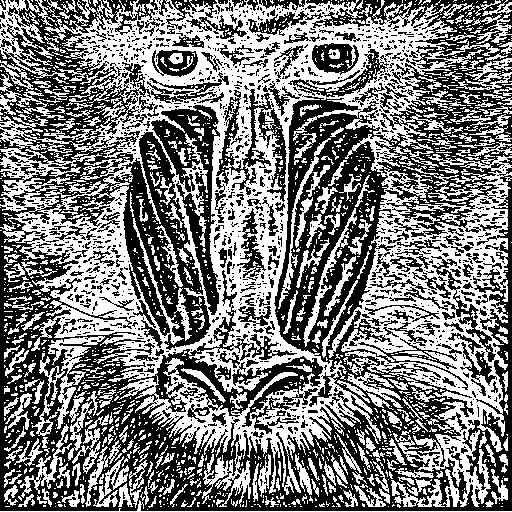
\includegraphics[width=0.3\hsize]{images/9x9-window/baboon_bernsen.png}
  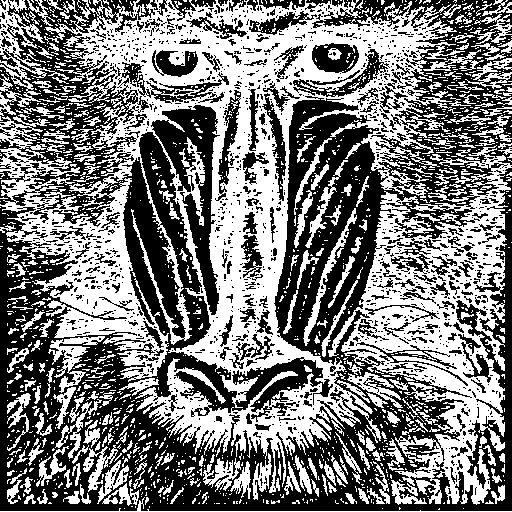
\includegraphics[width=0.3\hsize]{images/15x15-window/baboon_bernsen.png}
  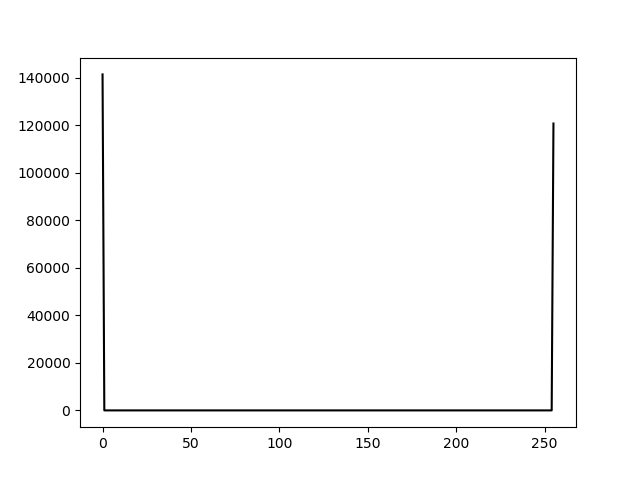
\includegraphics[width=0.3\hsize]{images/3x3-window/baboon_bernsen_histogram.png}
  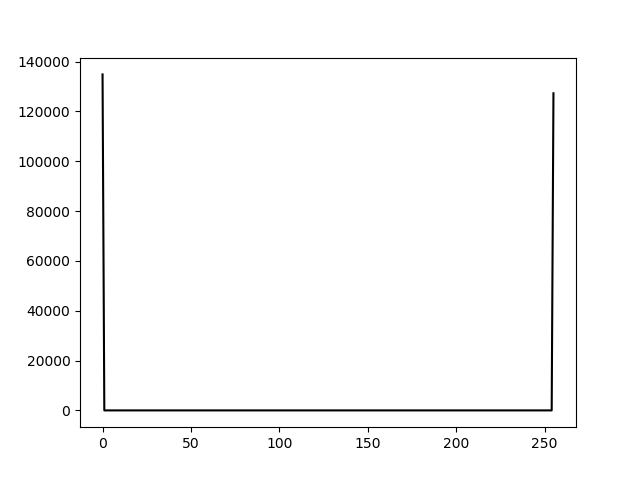
\includegraphics[width=0.3\hsize]{images/9x9-window/baboon_bernsen_histogram.png}
  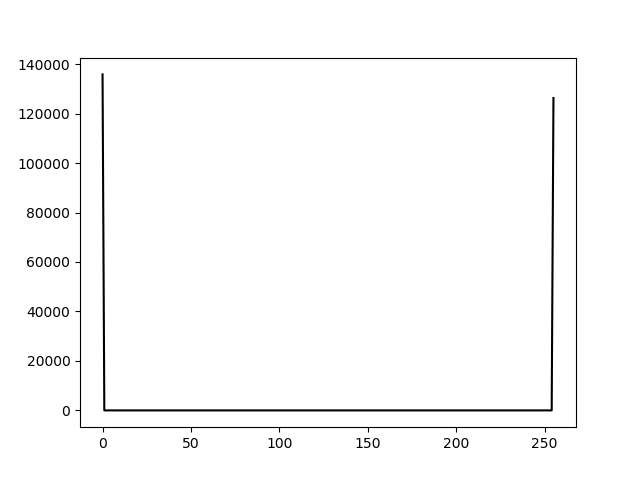
\includegraphics[width=0.3\hsize]{images/15x15-window//baboon_bernsen_histogram.png}
  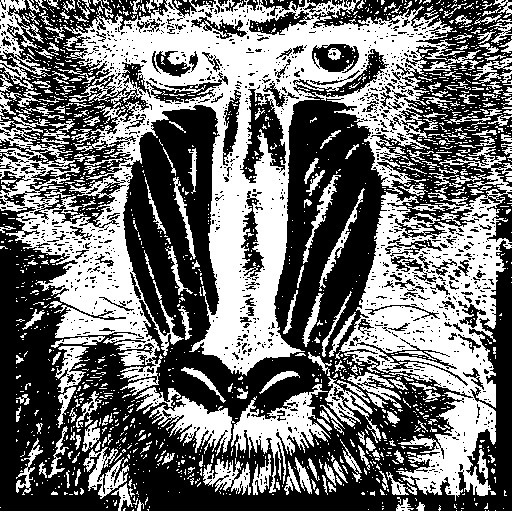
\includegraphics[width=0.3\hsize]{images/33x33-window/baboon_bernsen.png}
  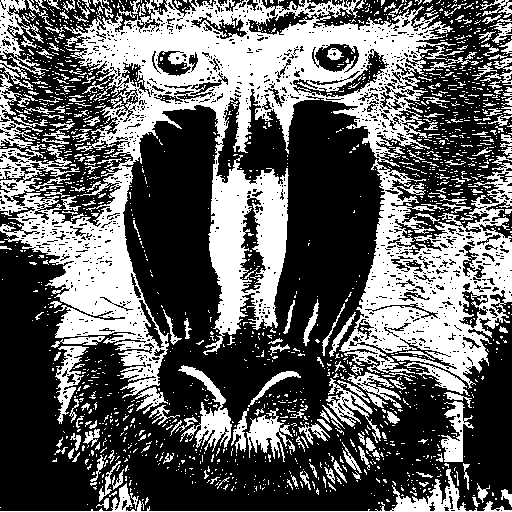
\includegraphics[width=0.3\hsize]{images/99x99-window/baboon_bernsen.png}
  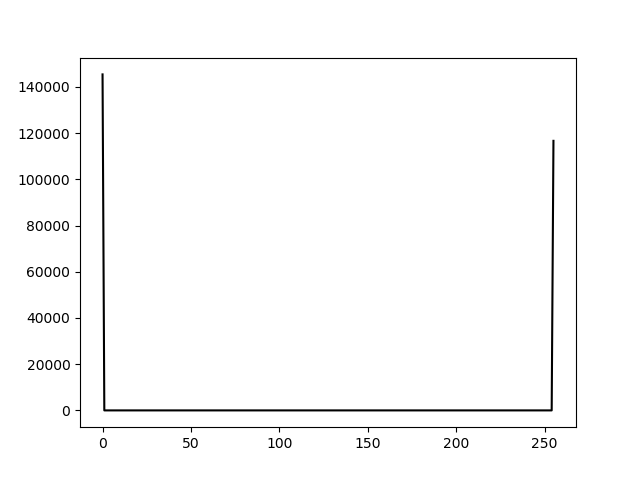
\includegraphics[width=0.4\hsize]{images/33x33-window/baboon_bernsen_histogram.png}
  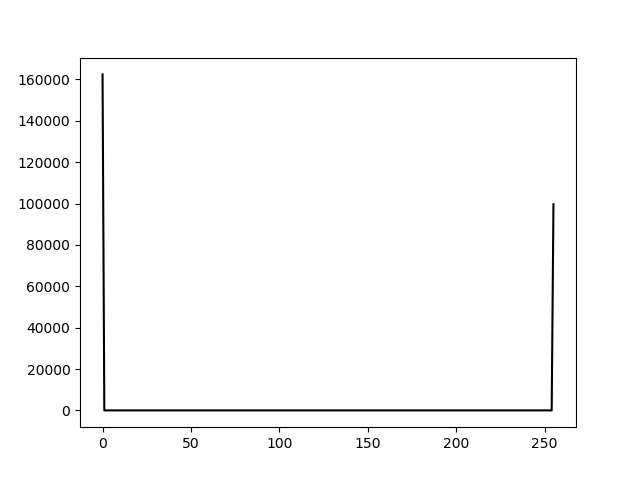
\includegraphics[width=0.4\hsize]{images/99x99-window/baboon_bernsen_histogram.png}
  \caption{Baboon images and histograms with local Bernsen threshold a) 3x3 neighborhood. b) 9x9 neighborhood. c) 15x15 neighborhood. d)Histogram for 3x3 neighborhood e)Histogram for 9x9 neighborhood f)Histogram for 15x15 neighborhood g) 33x33 neighborhood h) 99x99 neighborhood i) Histogram for 33x33 neighborhood. j) Histogram for 99x99 neighborhood}
  \label{fig:local-bernsen-baboon}
\end{figure}

\subsubsection{Niblack Method}
For the Niblack method, the Figure \ref{fig:local-niblack-fiducial} illustrates the obtained results for the fiducial image. As shown from the images and histograms, the bigger the window size, the more correct it is able to separate the object pixels from the background. In this case, for a small window (3x3), almost everything is an object. For the gib window (99x99), the objects are more noticeable, even though carrying error. 

\begin{figure}[h]
  \centering
  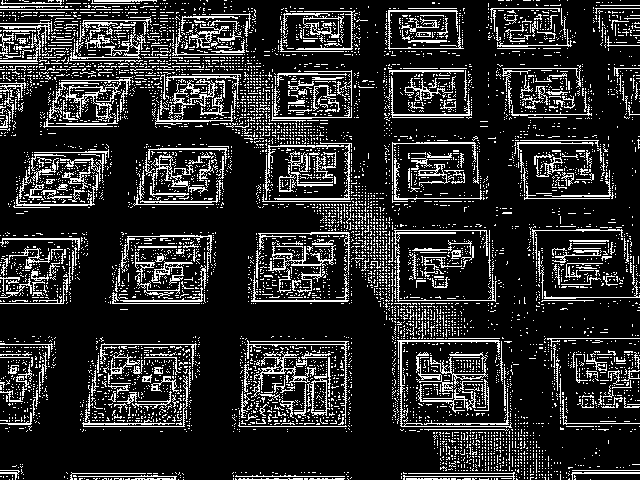
\includegraphics[width=0.3\hsize]{images/3x3-window/fiducial_niblack.png}
  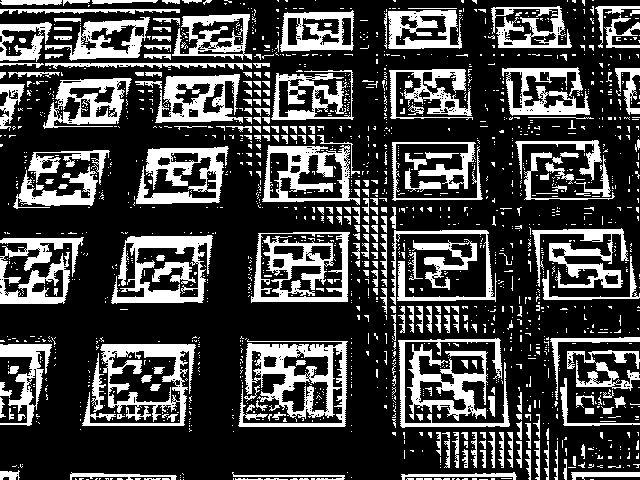
\includegraphics[width=0.3\hsize]{images/9x9-window/fiducial_niblack.png}
  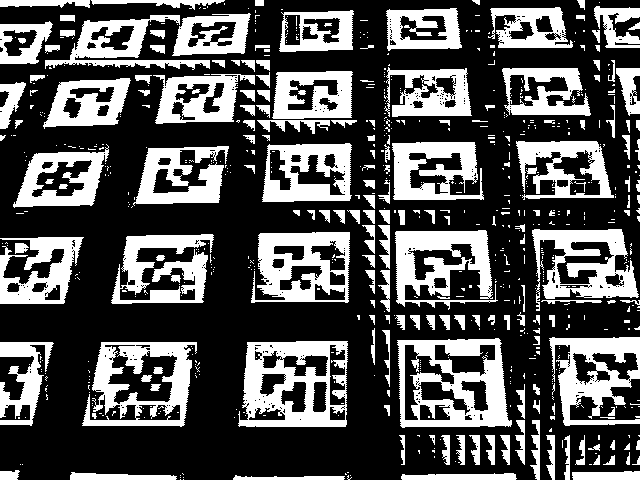
\includegraphics[width=0.3\hsize]{images/15x15-window/fiducial_niblack.png}
  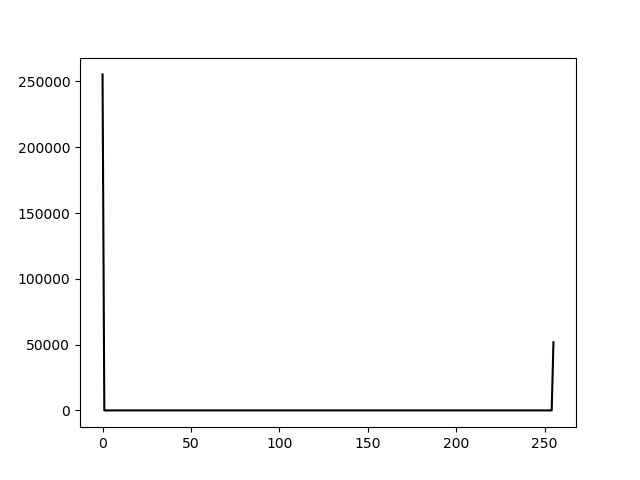
\includegraphics[width=0.3\hsize]{images/3x3-window/fiducial_niblack_histogram.png}
  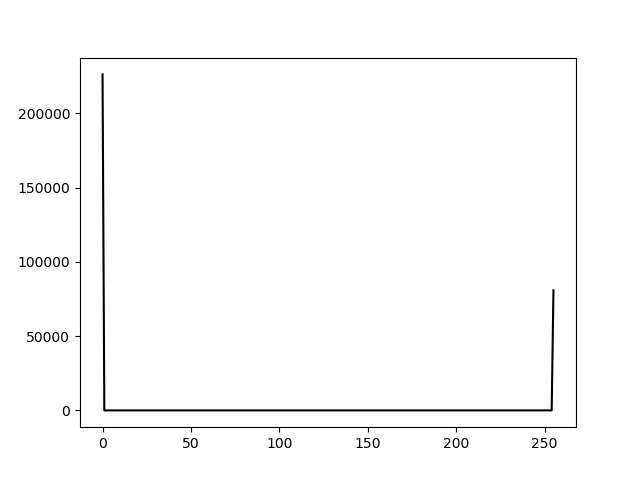
\includegraphics[width=0.3\hsize]{images/9x9-window/fiducial_niblack_histogram.png}
  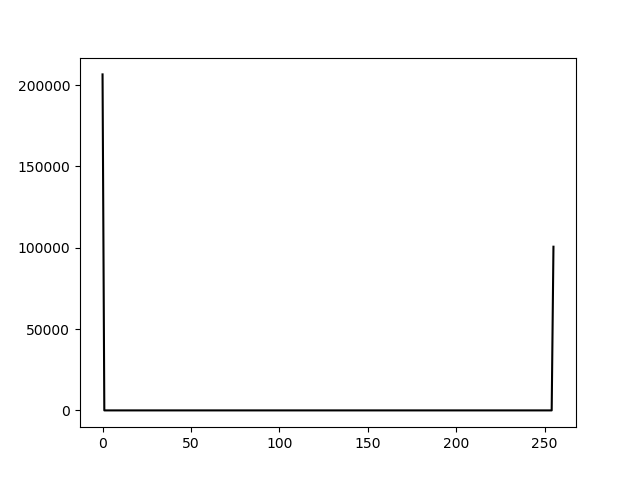
\includegraphics[width=0.3\hsize]{images/15x15-window//fiducial_niblack_histogram.png}
  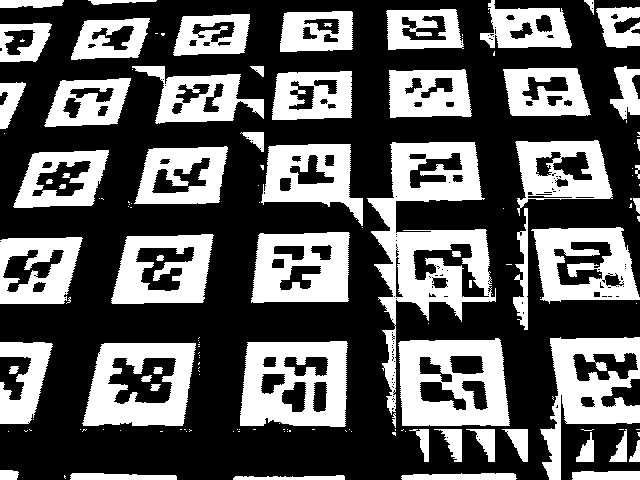
\includegraphics[width=0.3\hsize]{images/33x33-window/fiducial_niblack.png}
  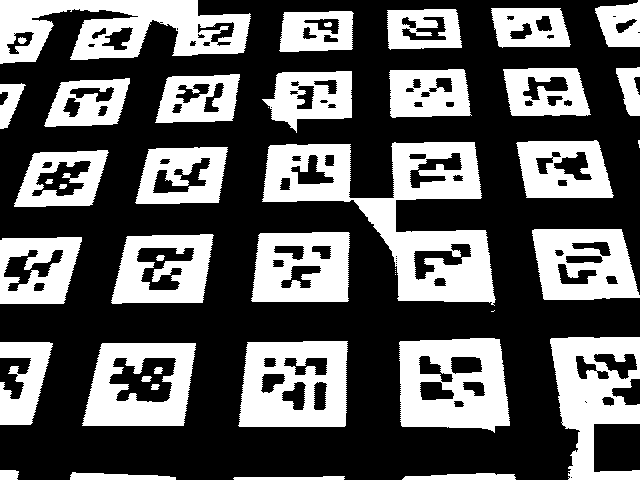
\includegraphics[width=0.3\hsize]{images/99x99-window/fiducial_niblack.png}
  \includegraphics[width=0.4\hsize]{images/33x33-window/fiducial_niblack_histogram.png}
  \includegraphics[width=0.4\hsize]{images/99x99-window/fiducial_niblack_histogram.png}
  \caption{fiducial images and histograms with local niblack threshold a) 3x3 neighborhood. b) 9x9 neighborhood. c) 15x15 neighborhood. d)Histogram for 3x3 neighborhood e)Histogram for 9x9 neighborhood f)Histogram for 15x15 neighborhood g) 33x33 neighborhood h) 99x99 neighborhood i) Histogram for 33x33 neighborhood. j) Histogram for 99x99 neighborhood}
  \label{fig:local-niblack-fiducial}
\end{figure}

\subsubsection{Sauvola and Pietaksinen Method}
For the Sauvola and Pietaksinen method, the Figure \ref{fig:local-sauvola-monarch} illustrates the obtained results for the monarch image. As shown from the images and histograms, the method inverted the background and the object, which is not the final objective (the obtained background are the leaves and the butterfly details, what would be desired to be the object). The bigger the window size, the more correct is the inversion.

\begin{figure}[h]
  \centering
  \includegraphics[width=0.3\hsize]{images/3x3-window/monarch_sauvola-pietaksinen.png}
  \includegraphics[width=0.3\hsize]{images/9x9-window/monarch_sauvola-pietaksinen.png}
  \includegraphics[width=0.3\hsize]{images/15x15-window/monarch_sauvola-pietaksinen.png}
  \includegraphics[width=0.3\hsize]{images/3x3-window/monarch_sauvola-pietaksinen_histogram.png}
  \includegraphics[width=0.3\hsize]{images/9x9-window/monarch_sauvola-pietaksinen_histogram.png}
  \includegraphics[width=0.3\hsize]{images/15x15-window//monarch_sauvola-pietaksinen_histogram.png}
  \includegraphics[width=0.3\hsize]{images/33x33-window/monarch_sauvola-pietaksinen.png}
  \includegraphics[width=0.3\hsize]{images/99x99-window/monarch_sauvola-pietaksinen.png}
  \includegraphics[width=0.4\hsize]{images/33x33-window/monarch_sauvola-pietaksinen_histogram.png}
  \includegraphics[width=0.4\hsize]{images/99x99-window/monarch_sauvola-pietaksinen_histogram.png}
  \caption{monarch images and histograms with local sauvola and pietaksinen threshold a) 3x3 neighborhood. b) 9x9 neighborhood. c) 15x15 neighborhood. d)Histogram for 3x3 neighborhood e)Histogram for 9x9 neighborhood f)Histogram for 15x15 neighborhood g) 33x33 neighborhood h) 99x99 neighborhood i) Histogram for 33x33 neighborhood. j) Histogram for 99x99 neighborhood}
  \label{fig:local-sauvola-monarch}
\end{figure}

\subsubsection{Phansalskar, More and Sabale Method}
For the Phansalskar, More and Sabale method, the Figure \ref{fig:local-more-peppers} illustrates the obtained results for the pepper image. As shown from the images and histograms, the smaller the neighborhood size, the better the results. The objects are well separated from the (little) background, and for bigger neighborhoods, the associated error is higher. 

\begin{figure}[h]
  \centering
  \includegraphics[width=0.3\hsize]{images/3x3-window/peppers_phansalskar-more-sabale.png}
  \includegraphics[width=0.3\hsize]{images/9x9-window/peppers_phansalskar-more-sabale.png}
  \includegraphics[width=0.3\hsize]{images/15x15-window/peppers_phansalskar-more-sabale.png}
  \includegraphics[width=0.3\hsize]{images/3x3-window/peppers_phansalskar-more-sabale_histogram.png}
  \includegraphics[width=0.3\hsize]{images/9x9-window/peppers_phansalskar-more-sabale_histogram.png}
  \includegraphics[width=0.3\hsize]{images/15x15-window//peppers_phansalskar-more-sabale_histogram.png}
  \includegraphics[width=0.3\hsize]{images/33x33-window/peppers_phansalskar-more-sabale.png}
  \includegraphics[width=0.3\hsize]{images/99x99-window/peppers_phansalskar-more-sabale.png}
  \includegraphics[width=0.4\hsize]{images/33x33-window/peppers_phansalskar-more-sabale_histogram.png}
  \includegraphics[width=0.4\hsize]{images/99x99-window/peppers_phansalskar-more-sabale_histogram.png}
  \caption{Peppers images and histograms with local Phansalskar, More and Sabale threshold a) 3x3 neighborhood. b) 9x9 neighborhood. c) 15x15 neighborhood. d)Histogram for 3x3 neighborhood e)Histogram for 9x9 neighborhood f)Histogram for 15x15 neighborhood g) 33x33 neighborhood h) 99x99 neighborhood i) Histogram for 33x33 neighborhood. j) Histogram for 99x99 neighborhood}
  \label{fig:local-more-peppers}
\end{figure}

\subsubsection{Contrast Method}
For the Contrast method, the Figure \ref{fig:local-contrast-retina} illustrates the obtained results for the retina image. As shown from the images and histograms, intermediate values of neighborhood sizes (like 9x9 and 15x15) have the better results. Smaller windows keeps to much of the background as the object. Bigger windows transforms part of the object into background. 

\begin{figure}[h]
  \centering
  \includegraphics[width=0.3\hsize]{images/3x3-window/retina_contrast.png}
  \includegraphics[width=0.3\hsize]{images/9x9-window/retina_contrast.png}
  \includegraphics[width=0.3\hsize]{images/15x15-window/retina_contrast.png}
  \includegraphics[width=0.3\hsize]{images/3x3-window/retina_contrast_histogram.png}
  \includegraphics[width=0.3\hsize]{images/9x9-window/retina_contrast_histogram.png}
  \includegraphics[width=0.3\hsize]{images/15x15-window//retina_contrast_histogram.png}
  \includegraphics[width=0.3\hsize]{images/33x33-window/retina_contrast.png}
  \includegraphics[width=0.3\hsize]{images/99x99-window/retina_contrast.png}
  \includegraphics[width=0.4\hsize]{images/33x33-window/retina_contrast_histogram.png}
  \includegraphics[width=0.4\hsize]{images/99x99-window/retina_contrast_histogram.png}
  \caption{Retina images and histograms with local Contrast threshold a) 3x3 neighborhood. b) 9x9 neighborhood. c) 15x15 neighborhood. d)Histogram for 3x3 neighborhood e)Histogram for 9x9 neighborhood f)Histogram for 15x15 neighborhood g) 33x33 neighborhood h) 99x99 neighborhood i) Histogram for 33x33 neighborhood. j) Histogram for 99x99 neighborhood}
  \label{fig:local-contrast-retina}
\end{figure}

\subsubsection{Mean Method}
For the Mean method, the Figure \ref{fig:local-mean-sonnet} illustrates the obtained results for the sonnet image. As shown from the images and histograms, intermediate values of neighborhood sizes (like 15x15) kept more the information to differentiate the background from the text. The method had poor performance for those types of images in general. 

\begin{figure}[h]
  \centering
  \includegraphics[width=0.3\hsize]{images/3x3-window/sonnet_mean.png}
  \includegraphics[width=0.3\hsize]{images/9x9-window/sonnet_mean.png}
  \includegraphics[width=0.3\hsize]{images/15x15-window/sonnet_mean.png}
  \includegraphics[width=0.3\hsize]{images/3x3-window/sonnet_mean_histogram.png}
  \includegraphics[width=0.3\hsize]{images/9x9-window/sonnet_mean_histogram.png}
  \includegraphics[width=0.3\hsize]{images/15x15-window//sonnet_mean_histogram.png}
  \includegraphics[width=0.3\hsize]{images/33x33-window/sonnet_mean.png}
  \includegraphics[width=0.3\hsize]{images/99x99-window/sonnet_mean.png}
  \includegraphics[width=0.4\hsize]{images/33x33-window/sonnet_mean_histogram.png}
  \includegraphics[width=0.4\hsize]{images/99x99-window/sonnet_mean_histogram.png}
  \caption{Sonnet images and histograms with local Mean threshold a) 3x3 neighborhood. b) 9x9 neighborhood. c) 15x15 neighborhood. d)Histogram for 3x3 neighborhood e)Histogram for 9x9 neighborhood f)Histogram for 15x15 neighborhood g) 33x33 neighborhood h) 99x99 neighborhood i) Histogram for 33x33 neighborhood. j) Histogram for 99x99 neighborhood}
  \label{fig:local-mean-sonnet}
\end{figure}

\subsubsection{Median Method}
For the Median method, the Figure \ref{fig:local-median-wedge} illustrates the obtained results for the wedge image. As shown from the images and histograms, smaller neighborhood sizes dealt better whent trying to locate the object borders within the image. Bigger window sizes lead to high associated error. 

\begin{figure}[h]
  \centering
  \includegraphics[width=0.3\hsize]{images/3x3-window/wedge_median.png}
  \includegraphics[width=0.3\hsize]{images/9x9-window/wedge_median.png}
  \includegraphics[width=0.3\hsize]{images/15x15-window/wedge_median.png}
  \includegraphics[width=0.3\hsize]{images/3x3-window/wedge_median_histogram.png}
  \includegraphics[width=0.3\hsize]{images/9x9-window/wedge_median_histogram.png}
  \includegraphics[width=0.3\hsize]{images/15x15-window//wedge_median_histogram.png}
  \includegraphics[width=0.3\hsize]{images/33x33-window/wedge_median.png}
  \includegraphics[width=0.3\hsize]{images/99x99-window/wedge_median.png}
  \includegraphics[width=0.4\hsize]{images/33x33-window/wedge_median_histogram.png}
  \includegraphics[width=0.4\hsize]{images/99x99-window/wedge_median_histogram.png}
  \caption{Wedge images and histograms with local Median threshold a) 3x3 neighborhood. b) 9x9 neighborhood. c) 15x15 neighborhood. d)Histogram for 3x3 neighborhood e)Histogram for 9x9 neighborhood f)Histogram for 15x15 neighborhood g) 33x33 neighborhood h) 99x99 neighborhood i) Histogram for 33x33 neighborhood. j) Histogram for 99x99 neighborhood}
  \label{fig:local-median-wedge}
\end{figure}

\subsection{Local Methods Comparisons}

In this subsection the methods are compared, trying to analyze their best results for every input image, independent of neighborhood size.

\subsubsection{Baboon Image}

As it can be seen from figure \ref{fig:local-baboon}, most of the methods are able to separate the details of the baboon, with good results for Bernsen method. The 15x15 neighborhood had the better results overall.

\begin{figure}[h]
  \centering
  \includegraphics[width=0.3\hsize]{images/15x15-window/baboon_bernsen.png}
  \includegraphics[width=0.3\hsize]{images/15x15-window/baboon_niblack.png}
  \includegraphics[width=0.3\hsize]{images/99x99-window/baboon_sauvola-pietaksinen.png}
  \includegraphics[width=0.3\hsize]{images/15x15-window/baboon_bernsen_histogram.png}
  \includegraphics[width=0.3\hsize]{images/15x15-window/baboon_niblack_histogram.png}
  \includegraphics[width=0.3\hsize]{images/99x99-window//baboon_sauvola-pietaksinen_histogram.png}
  \includegraphics[width=0.3\hsize]{images/99x99-window/baboon_phansalskar-more-sabale.png}
  \includegraphics[width=0.3\hsize]{images/15x15-window/baboon_contrast.png}
  \includegraphics[width=0.3\hsize]{images/15x15-window/baboon_mean.png}
  \includegraphics[width=0.3\hsize]{images/99x99-window/baboon_phansalskar-more-sabale_histogram.png}
  \includegraphics[width=0.3\hsize]{images/15x15-window/baboon_contrast_histogram.png}
  \includegraphics[width=0.3\hsize]{images/15x15-window/baboon_mean_histogram.png}
  \includegraphics[width=0.3\hsize]{images/15x15-window/baboon_median.png}
  \includegraphics[width=0.3\hsize]{images/15x15-window/baboon_median_histogram.png}

  \caption{Baboon images and histograms with different methods a) 15x15 neighborhood, Bernsen. b) 15x15 neighborhood, Niblack. c) 99x99 neighborhood, Sauvola and Pietaksinen. d)Histogram for 15x15 neighborhood, Bernsen e)Histogram for 15x15 neighborhood, Niblack f)Histogram for 99x99 neighborhood, Sauvola and Pietaksinen g) 99x99 neighborhood, Phansalskar, More and Sabale h) 15x15 neighborhood, Contrast i) 15x15 neighborhood, Mean j) Histogram for 99x99 neighborhood, Phansalskar, More and Sabale. k) Histogram for 15x15 neighborhood, Contrast l) Histogram for 15x15 neighborhood, Mean m) 15x15 neighborhood, Median n) Histogram for 15x15 neighborhood, Median}
  \label{fig:local-baboon}
\end{figure}

\subsubsection{Fiducial Image}
As it can be seen from figure \ref{fig:local-fiducial}, most of the methods are able to separate the details from the image, even with the presence of shading,   with the Sauvola and Pietaksinen method with the best results. The better results were obtained using higher neighborhood sizes (mostly 99x99).

\begin{figure}[h]
  \centering
  \includegraphics[width=0.3\hsize]{images/33x33-window/fiducial_bernsen.png}
  \includegraphics[width=0.3\hsize]{images/99x99-window/fiducial_niblack.png}
  \includegraphics[width=0.3\hsize]{images/99x99-window/fiducial_sauvola-pietaksinen.png}
  \includegraphics[width=0.3\hsize]{images/33x33-window/fiducial_bernsen_histogram.png}
  \includegraphics[width=0.3\hsize]{images/99x99-window/fiducial_niblack_histogram.png}
  \includegraphics[width=0.3\hsize]{images/99x99-window//fiducial_sauvola-pietaksinen_histogram.png}
  \includegraphics[width=0.3\hsize]{images/99x99-window/fiducial_phansalskar-more-sabale.png}
  \includegraphics[width=0.3\hsize]{images/33x33-window/fiducial_contrast.png}
  \includegraphics[width=0.3\hsize]{images/99x99-window/fiducial_mean.png}
  \includegraphics[width=0.3\hsize]{images/99x99-window/fiducial_phansalskar-more-sabale_histogram.png}
  \includegraphics[width=0.3\hsize]{images/33x33-window/fiducial_contrast_histogram.png}
  \includegraphics[width=0.3\hsize]{images/99x99-window/fiducial_mean_histogram.png}
  \includegraphics[width=0.3\hsize]{images/99x99-window/fiducial_median.png}
  \includegraphics[width=0.3\hsize]{images/99x99-window/fiducial_median_histogram.png}

  \caption{Fiducial images and histograms with different methods a) 33x33 neighborhood, Bernsen. b) 99x99 neighborhood, Niblack. c) 99x99 neighborhood, Sauvola and Pietaksinen. d)Histogram for 33x33 neighborhood, Bernsen e)Histogram for 99x99 neighborhood, Niblack f)Histogram for 99x99 neighborhood, Sauvola and Pietaksinen g) 99x99 neighborhood, Phansalskar, More and Sabale h) 33x33 neighborhood, Contrast i) 99x99 neighborhood, Mean j) Histogram for 99x99 neighborhood, Phansalskar, More and Sabale. k) Histogram for 33x33 neighborhood, Contrast l) Histogram for 99x99 neighborhood, Mean m) 99x99 neighborhood, Median n) Histogram for 99x99 neighborhood, Median}
  \label{fig:local-fiducial}
\end{figure}

\subsubsection{Monarch Image}
For the Monarch image (figure \ref{fig:local-monarch}), the methods, except for Sauvola and Pietaksinen (inverted results), had trouble to separate the objetcs from the background. Bernsen has interesting result, as it isolates the butterfly and leaves area. If consider the inverted result of Sauvola and Pietaksinen, it would give the better results. The higher neighborhood windows gave the best results for every method.

\begin{figure}[h]
  \centering
  \includegraphics[width=0.3\hsize]{images/99x99-window/monarch_bernsen.png}
  \includegraphics[width=0.3\hsize]{images/99x99-window/monarch_niblack.png}
  \includegraphics[width=0.3\hsize]{images/99x99-window/monarch_sauvola-pietaksinen.png}
  \includegraphics[width=0.3\hsize]{images/99x99-window/monarch_bernsen_histogram.png}
  \includegraphics[width=0.3\hsize]{images/99x99-window/monarch_niblack_histogram.png}
  \includegraphics[width=0.3\hsize]{images/99x99-window//monarch_sauvola-pietaksinen_histogram.png}
  \includegraphics[width=0.3\hsize]{images/99x99-window/monarch_phansalskar-more-sabale.png}
  \includegraphics[width=0.3\hsize]{images/99x99-window/monarch_contrast.png}
  \includegraphics[width=0.3\hsize]{images/99x99-window/monarch_mean.png}
  \includegraphics[width=0.3\hsize]{images/99x99-window/monarch_phansalskar-more-sabale_histogram.png}
  \includegraphics[width=0.3\hsize]{images/99x99-window/monarch_contrast_histogram.png}
  \includegraphics[width=0.3\hsize]{images/99x99-window/monarch_mean_histogram.png}
  \includegraphics[width=0.3\hsize]{images/99x99-window/monarch_median.png}
  \includegraphics[width=0.3\hsize]{images/99x99-window/monarch_median_histogram.png}

  \caption{Monarch images and histograms with different methods a) 99x99 neighborhood, Bernsen. b) 99x99 neighborhood, Niblack. c) 99x99 neighborhood, Sauvola and Pietaksinen. d)Histogram for 99x99 neighborhood, Bernsen e)Histogram for 99x99 neighborhood, Niblack f)Histogram for 99x99 neighborhood, Sauvola and Pietaksinen g) 99x99 neighborhood, Phansalskar, More and Sabale h) 99x99 neighborhood, Contrast i) 99x99 neighborhood, Mean j) Histogram for 99x99 neighborhood, Phansalskar, More and Sabale. k) Histogram for 99x99 neighborhood, Contrast l) Histogram for 99x99 neighborhood, Mean m) 99x99 neighborhood, Median n) Histogram for 99x99 neighborhood, Median}
  \label{fig:local-monarch}
\end{figure}

\subsubsection{Peppers Image}
For the Peppers image (high contrast), showed in figure \ref{fig:local-peppers}, the Sauvola and Pietaksinen and Phansalskar, More and Sabale manage to separate the objects from the background with great results. The other methods had trouble to do so. The window sizes vary by method. Small windows produced optimal results for Phansalskar et al.

\begin{figure}[h]
  \centering
  \includegraphics[width=0.3\hsize]{images/15x15-window/peppers_bernsen.png}
  \includegraphics[width=0.3\hsize]{images/15x15-window/peppers_niblack.png}
  \includegraphics[width=0.3\hsize]{images/99x99-window/peppers_sauvola-pietaksinen.png}
  \includegraphics[width=0.3\hsize]{images/15x15-window/peppers_bernsen_histogram.png}
  \includegraphics[width=0.3\hsize]{images/15x15-window/peppers_niblack_histogram.png}
  \includegraphics[width=0.3\hsize]{images/99x99-window//peppers_sauvola-pietaksinen_histogram.png}
  \includegraphics[width=0.3\hsize]{images/3x3-window/peppers_phansalskar-more-sabale.png}
  \includegraphics[width=0.3\hsize]{images/9x9-window/peppers_contrast.png}
  \includegraphics[width=0.3\hsize]{images/9x9-window/peppers_mean.png}
  \includegraphics[width=0.3\hsize]{images/3x3-window/peppers_phansalskar-more-sabale_histogram.png}
  \includegraphics[width=0.3\hsize]{images/9x9-window/peppers_contrast_histogram.png}
  \includegraphics[width=0.3\hsize]{images/9x9-window/peppers_mean_histogram.png}
  \includegraphics[width=0.3\hsize]{images/15x15-window/peppers_median.png}
  \includegraphics[width=0.3\hsize]{images/15x15-window/peppers_median_histogram.png}

  \caption{Peppers images and histograms with different methods a) 15x15 neighborhood, Bernsen. b) 15x15 neighborhood, Niblack. c) 99x99 neighborhood, Sauvola and Pietaksinen. d)Histogram for 15x15 neighborhood, Bernsen e)Histogram for 15x15 neighborhood, Niblack f)Histogram for 99x99 neighborhood, Sauvola and Pietaksinen g) 99x99 neighborhood, Phansalskar, More and Sabale h) 9x9 neighborhood, Contrast i) 9x9 neighborhood, Mean j) Histogram for 99x99 neighborhood, Phansalskar, More and Sabale. k) Histogram for 9x9 neighborhood, Contrast l) Histogram for 9x9 neighborhood, Mean m) 15x15 neighborhood, Median n) Histogram for 15x15 neighborhood, Median}
  \label{fig:local-peppers}
\end{figure}

\subsubsection{Retina Image}
The results were various for the Retina image, as shown in figure \ref{fig:local-retina}. Bernsen and Contrast methods gave good results for separating the objects from the background. Medium size neighborhoods performed better for the methods for this image.

\begin{figure}[h]
  \centering
  \includegraphics[width=0.3\hsize]{images/9x9-window/retina_bernsen.png}
  \includegraphics[width=0.3\hsize]{images/33x33-window/retina_niblack.png}
  \includegraphics[width=0.3\hsize]{images/99x99-window/retina_sauvola-pietaksinen.png}
  \includegraphics[width=0.3\hsize]{images/9x9-window/retina_bernsen_histogram.png}
  \includegraphics[width=0.3\hsize]{images/33x33-window/retina_niblack_histogram.png}
  \includegraphics[width=0.3\hsize]{images/99x99-window//retina_sauvola-pietaksinen_histogram.png}
  \includegraphics[width=0.3\hsize]{images/15x15-window/retina_phansalskar-more-sabale.png}
  \includegraphics[width=0.3\hsize]{images/15x15-window/retina_contrast.png}
  \includegraphics[width=0.3\hsize]{images/15x15-window/retina_mean.png}
  \includegraphics[width=0.3\hsize]{images/15x15-window/retina_phansalskar-more-sabale_histogram.png}
  \includegraphics[width=0.3\hsize]{images/15x15-window/retina_contrast_histogram.png}
  \includegraphics[width=0.3\hsize]{images/15x15-window/retina_mean_histogram.png}
  \includegraphics[width=0.3\hsize]{images/99x99-window/retina_median.png}
  \includegraphics[width=0.3\hsize]{images/99x99-window/retina_median_histogram.png}

  \caption{Retina images and histograms with different methods a) 9x9 neighborhood, Bernsen. b) 33x33 neighborhood, Niblack. c) 99x99 neighborhood, Sauvola and Pietaksinen. d)Histogram for 9x9 neighborhood, Bernsen e)Histogram for 33x33 neighborhood, Niblack f)Histogram for 99x99 neighborhood, Sauvola and Pietaksinen g) 15x15 neighborhood, Phansalskar, More and Sabale h) 15x15 neighborhood, Contrast i) 15x15 neighborhood, Mean j) Histogram for 15x15 neighborhood, Phansalskar, More and Sabale. k) Histogram for 15x15 neighborhood, Contrast l) Histogram for 15x15 neighborhood, Mean m) 99x99 neighborhood, Median n) Histogram for 99x99 neighborhood, Median}
  \label{fig:local-retina}
\end{figure}

\subsubsection{Sonnet Image}
For the Sonnet image, ehich contains text, the methodologies implemented produce various results, as shown in figure \ref{fig:local-sonnet}. The best results were obtained by Bernsen and Phansalskar, More and Sabale, being able to distinguish the text from the paper, even bad lighting in the image. 

\begin{figure}[h]
  \centering
  \includegraphics[width=0.3\hsize]{images/99x99-window/sonnet_bernsen.png}
  \includegraphics[width=0.3\hsize]{images/9x9-window/sonnet_niblack.png}
  \includegraphics[width=0.3\hsize]{images/99x99-window/sonnet_sauvola-pietaksinen.png}
  \includegraphics[width=0.3\hsize]{images/99x99-window/sonnet_bernsen_histogram.png}
  \includegraphics[width=0.3\hsize]{images/9x9-window/sonnet_niblack_histogram.png}
  \includegraphics[width=0.3\hsize]{images/99x99-window//sonnet_sauvola-pietaksinen_histogram.png}
  \includegraphics[width=0.3\hsize]{images/33x33-window/sonnet_phansalskar-more-sabale.png}
  \includegraphics[width=0.3\hsize]{images/99x99-window/sonnet_contrast.png}
  \includegraphics[width=0.3\hsize]{images/33x33-window/sonnet_mean.png}
  \includegraphics[width=0.3\hsize]{images/33x33-window/sonnet_phansalskar-more-sabale_histogram.png}
  \includegraphics[width=0.3\hsize]{images/99x99-window/sonnet_contrast_histogram.png}
  \includegraphics[width=0.3\hsize]{images/33x33-window/sonnet_mean_histogram.png}
  \includegraphics[width=0.3\hsize]{images/99x99-window/sonnet_median.png}
  \includegraphics[width=0.3\hsize]{images/99x99-window/sonnet_median_histogram.png}

  \caption{Sonnet images and histograms with different methods a) 99x99 neighborhood, Bernsen. b) 9x9 neighborhood, Niblack. c) 99x99 neighborhood, Sauvola and Pietaksinen. d)Histogram for 99x99 neighborhood, Bernsen e)Histogram for 9x9 neighborhood, Niblack f)Histogram for 99x99 neighborhood, Sauvola and Pietaksinen g) 33x33 neighborhood, Phansalskar, More and Sabale h) 99x99 neighborhood, Contrast i) 33x33 neighborhood, Mean j) Histogram for 33x33 neighborhood, Phansalskar, More and Sabale. k) Histogram for 99x99 neighborhood, Contrast l) Histogram for 33x33 neighborhood, Mean m) 99x99 neighborhood, Median n) Histogram for 99x99 neighborhood, Median}
  \label{fig:local-sonnet}
\end{figure}

\subsubsection{Wedge Image}
The results for this image are shown in \ref{fig:local-wedge}. Even though good results were obtained for Bernsen and Contrast methods, Sauvola and Pietaksinen proved to be innefective for this image, probably due to bad lighting and contrast. 

\begin{figure}[h]
  \centering
  \includegraphics[width=0.3\hsize]{images/99x99-window/wedge_bernsen.png}
  \includegraphics[width=0.3\hsize]{images/99x99-window/wedge_niblack.png}
  \includegraphics[width=0.3\hsize]{images/99x99-window/wedge_sauvola-pietaksinen.png}
  \includegraphics[width=0.3\hsize]{images/99x99-window/wedge_bernsen_histogram.png}
  \includegraphics[width=0.3\hsize]{images/99x99-window/wedge_niblack_histogram.png}
  \includegraphics[width=0.3\hsize]{images/99x99-window//wedge_sauvola-pietaksinen_histogram.png}
  \includegraphics[width=0.3\hsize]{images/99x99-window/wedge_phansalskar-more-sabale.png}
  \includegraphics[width=0.3\hsize]{images/99x99-window/wedge_contrast.png}
  \includegraphics[width=0.3\hsize]{images/99x99-window/wedge_mean.png}
  \includegraphics[width=0.3\hsize]{images/99x99-window/wedge_phansalskar-more-sabale_histogram.png}
  \includegraphics[width=0.3\hsize]{images/99x99-window/wedge_contrast_histogram.png}
  \includegraphics[width=0.3\hsize]{images/99x99-window/wedge_mean_histogram.png}
  \includegraphics[width=0.3\hsize]{images/99x99-window/wedge_median.png}
  \includegraphics[width=0.3\hsize]{images/99x99-window/wedge_median_histogram.png}

  \caption{Wedge images and histograms with different methods a) 99x99 neighborhood, Bernsen. b) 99x99 neighborhood, Niblack. c) 99x99 neighborhood, Sauvola and Pietaksinen. d)Histogram for 99x99 neighborhood, Bernsen e)Histogram for 99x99 neighborhood, Niblack f)Histogram for 99x99 neighborhood, Sauvola and Pietaksinen g) 99x99 neighborhood, Phansalskar, More and Sabale h) 99x99 neighborhood, Contrast i) 99x99 neighborhood, Mean j) Histogram for 99x99 neighborhood, Phansalskar, More and Sabale. k) Histogram for 99x99 neighborhood, Contrast l) Histogram for 99x99 neighborhood, Mean m) 99x99 neighborhood, Median n) Histogram for 99x99 neighborhood, Median}
  \label{fig:local-wedge}
\end{figure}

\section{Conclusion}
The application of thresholding techniques to separate pixels from background and objects for future segmentation was possible thanks to the approaches presented in the academia.

The usage of different input images, thresholds and neighborhood sizes made it possible to analyze each approach's strength.

\end{document}
